\chapter{Flexibility}
\label{chap:Flexibility}

\emph{``You must be shapeless, formless, like water. When you pour water in a
cup, it becomes the cup. When you pour water in a bottle, it becomes the
bottle. When you pour water in a teapot, it becomes the teapot. Water can drip
and it can crash. Become like water my friend.''}

--- Bruce Lee \\

Any system exhibits particular compromises between opposing goals. Some
constraints derive from the nature of the problem a particular system is trying
to solve. Different problems might have conflicting constraints. Therefore, a
given system cannot be the ultimate answer to life, the universe and everything
to everybody. It follows that to assert the flexibility of a system, we need to
choose particular use cases and leave others.

The prospect of using the development of the system to drive requirements is
alluring, especially as a requirement analogy to the meta-circularity of the
system. However, we need to keep in mind that it is not sufficient to ensure
that the resulting system is more than a research curiosity. The following
usages are outgrowths of discussions that happened with Bruno Dufour to
determine usage scenarii that were less biaised by my own view of what the
system could be used for.

The single strategy behind every scenario is to define a protocol to implement
the element of interest and expose the parts that can vary as a method, which
can be replaced by user code. To emphasize the non-universal nature of a
particular solution, each scenario describes the modification made to the
system presented in the design section (see Section~\ref{chap:Design}).  This
is a deliberate choice to illustrate that flexibility is also enabled by having
clear lines of evolution around a unifying principle, in this case,
message-passing.

We first explore simple examples that work without modification to the
protocols of the system, to obtain profiling information in terms of JS operations.
We then discuss circumscribed modifications to the system, to enforce runtime
invariants used to catch common programming mistakes. We conclude with a more
involved example to provide fundational tools for dynamic analysis of JS code.

\section{Obtaining semantic-level profiling information}

Given a good approximation of the performance cost of JS operations, such as
property accesses and object creation, we might be interested in estimating the
performance of an application by computing the run-time frequency of each of
these operations.

The design of the system makes it easy to do by wrapping the method
implementing the semantic operation with a function incrementing a counter.
Instrumenting the property access (\kw{\_\_get\_\_}) might be done in the
following way:

\jsfile{listings/getcount.js}

Notice that the instrumentation can be granular both in time and space, i.e. it
can cover only a part of the execution and a subset of all the objects present
in the system. In the preceding example, it is only performed on the \kw{o}
object. To cover the entire application execution, instrumentation can be performed before
an application is actually started. To cover all objects of a given type, such
as all functions, the corresponding root object method can be instrumented.

The same pattern can be applied to object creation by instrumenting the
\kw{\_\_new\_\_} operation instead.


\section{Verifying runtime invariants}

The preceding examples were implemented by wrapping the existing method with
another one to allow pre and post treatment around the original operation. The
next examples \textit{modifies} the semantic of the original operation to
provide a different behavior.

\subsection{Ensure that all accesses are made to existing properties}

The default semantic of property access in JS specifies that accessing
a non-existing property should return \kw{undefined}. It has the unfortunate
consequence that the presence or absence of a property on an object is
ambiguous: if an existing property has \kw{undefined} as a value, we cannot
tell if the property is present or not by the return value of the property
access operation. Combined with the automatic conversion of values for most
operations, an unintended missing property on an object might cause obscure
bugs to crop up later in the program.

We can provide a \textit{fail early} semantic to the property access operation
by raising an exception if a property is not present. This can be done easily 
by replacing the \kw{\_\_get\_\_} operation on the root object:

\jsfile{listings/failearlyget.js}

In this example, to implement the semantic of the property access, we need
access to the underlying object representation. For this example, we do it by
specifying directly the code that should be generated as a string. The map
property lookup operation returns \kw{undefined} if the property is not present
on a given object. If no object in the prototype chain has the property, the
while loop will end and an exception will be thrown.  Notably, having separate
cases for the presence of a property with an \kw{undefined} value and an absent
property, an exception can be thrown only in the second case.

A similar method could be used to check arrays for out-of-bounds accesses by redefining
the \kw{__get__} method of the root array.

As a side note, the convenience of syntactic support would greatly help
readability for specifying the semantic in terms of the underlying
representation but it is orthogonal to the issue of being able to redefine the
semantic of an operation. It is therefore left as future work.

\subsection{Ensure that a constructor always returns the object it received}

The semantic of object construction in JS can be surprising. When creating an
object with a call to a function with the \kw{new} operator, a new empty object
is created behind the scene and the function will be called with a \kw{this}
value bound to the created object. When the function returns, the return value type 
is inspected. If it is an object, the \kw{new} expression will yield the
returned object. However, if it is a primitive value, the \kw{new} expression
will yield the object created before the call to the function.

This behavior guarantees that an object will always be returned and allows
constructors to be written more succintly by omitting the \kw{return}
statement. However, it might also be a source of run-time errors if a
constructor is later modified and an object is unintentionnally returned.

To catch that kind of error, we can expose a construction protocol for
functions. The basic idea is to convert all constructor calls made with the new
operator, for example \kw{new Foo()}, to a call to a special purpose method,
such as \kw{Foo.__ctor__()}.

This requires a modification of the compiler. The simplest way to do it with
the current compiler is to modify the desugaring of the new operator. It also
requires an implementation of the construction protocol. A simple
implementation is given, using implementation-level JS:

\jsfile{listings/ctor.js}

Given this implementation, we can dynamically change the semantic of the
construction operation to throw an error if an object different than the
orignal object created is returned by the constructor the following way:

\jsfile{listings/constructorcheck.js}

This implementation assumes that all constructors do not use parameters. A
complete implementation would need to use the \kw{arguments} object to pass the
arguments received to the function called. This is omitted here for simplicity.

\section{Avoiding profiling the profiling code}

This last example is a little more involved. It illustrates how JS can be used
to accumulate substantial information on a running JS program. The main issue
it raises is how to avoid profiling the profiling code when it is written in
the same language as the profiled code. Conceptually, we would like the
profiling code to execute in a different environment than the profiled code.
The usual approach is to protect the profiling code in a \textit{critical
section} that deactivate profiling for that part of the execution. This section
illustrates two additional techniques that are available to a meta-circular
system. 

The first one is analoguous to the use of a different language in the
implementation of a VM and consist in writing the profiling code in the
implementation-level JS. The similarity of languages allows objects to be
shared between both levels although some conversions must be performed at the
boundary. 

The second one is based on the idea of providing a separate object model to the
profiling code. It consists in effectively providing a different run-time
environment with the benefit that the objects of this second environment are
entirely compatible with the first one, i.e. they follow the same calling
convention, protocols and layout, allowing them to be stored in objects of
other environments and inversely. Since the root objects for objects of
different environments are different, modifying the root objects' methods
changes the behavior of objects only in the same environment, providing
granularity of profiling while maintaining uniformity and avoiding difficulting
in reasoning about critical sections. I believe it is an original contribution.

We will see the three techniques applied to the task of obtaining a dynamic
call graph. The problem of obtaining a dynamic call graph is explained and a
sample program is introduced, the requirements made on the VM are given and
finally the three techniques are presented.

\subsection{Obtaining a dynamic call graph}

A dynamic call graph is a data structure encoding the calling relationship
between functions, occurring during the execution of a program. For example, if
a function \kw{a} calls a function \kw{b}, the \textit{a calls b} relationship
will be registered in some way. For context-insensitive call graphs, we might
represent functions as nodes and calling relationships as edges.
Context-sentitive call graphs could represent functions as multiple nodes,
depending on their respective callers. For the sake of simplicity, we will
consider a context-insensitive call graph for the remainder of this example. 

Dynamic call graphs can be used to determine the code coverage of unit tests,
to provide detailed runtime information for code comprehension and can provide
information for run-time optimizations and to provide basic information on which
analysis can run.

% Instrumentation points at the semantic level of JS
To obtain that information we need to instrument every operation that result in
a function call in JS:
\begin{enumerate}
    \item Global function calls
    \item Method calls made on objects
    \item Indirect calls made through \kw{call} and \kw{apply} 
    \item Direct call of functions stored in variables
\end{enumerate}

The following program will be analysed and exhibits every case enumerated
above. Four different functions are declared and two are initially called:

\jsfile{listings/callgraphexample.js}

By inspection, we can see that \kw{a} calls \kw{b}, that \kw{b} calls no other
function, that \kw{c} recursively calls itself but no other function and \kw{d}
is not called nor calls another function. We would expect a call graph like the
one shown in Figure~\ref{fig:CallGraph} to modelize those relationships.

\begin{figure}[htb]
\begin{center}
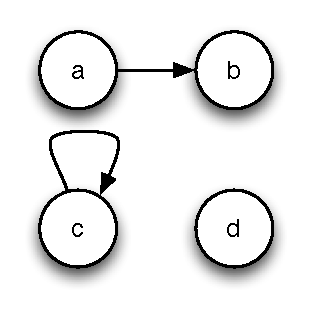
\includegraphics{figures/callgraph}
\caption{\label{fig:CallGraph} Call Graph for example code}
\end{center}
\end{figure}

Our design makes the instrumentation easy. Global functions are considered
methods and are therefore handled with the same mecanism as methods. Method
calls can be intercepted through a lookup protocol. Indirect calls can be
intercepted by wrapping the \kw{call} and \kw{apply} methods. Direct calls can
be intercepted by forcing every function to be called through its \kw{call}
method.

A context-insensitive analysis requires a single node by function. Therefore,
we can store the profiling information directly on the functions themselves.
This way it avoids the complexity associated with maintaining separate data
structures and maintaining a correspondance between functions and those data
structures.

Some minor modifications are required to the compiler, especially to support
the fourth case. These modifications are sufficient to provide the
instrumentation hooks required to obtain a dynamic call graph. The next
sections explain different strategy for writing the profiling code and their
pitfalls.

\subsection{Protecting the profiling code in a critical section} 

A \textit{critical section} usually refers to a section of code in a
multi-threaded program in which the system guarantees that no preemption will
occur. By analogy, we use the term to refer to a section of code in a profiled
program in which the system guarantees that no profiling occurs.

By using a critical section, we solve the issue of having the profiling code
being profiled. It is important to avoid profiling the profiling code, not only
because it pollutes results but mostly because it can introduce
\textit{meta-stability} issues, namely that performing an operation in the
profiling code might call back into the same operation being profiled, creating
an infinite loop.

A critical section can be implemented by introducing a flag that controls
whether profiling occurs or not. Just before the profiling code starts
executing, the flag is set and right after the profiling code ends the flag is
reset. It can be done with a boolean variable if the section needs not be
reentrant or with a integer otherwise.

When profiling JS function calls, we need to be cautious about the different
ways the flow of control can be manipulated by the callee. In JS, a function
can return either normally through its explicit or implicit return statement or
by raising an exception. Fortunately, JS provides a \kw{finally} construct that
garantees that however a function returns, the \kw{finally} block will always
be executed. We can therefore perform pre-call operations in a \kw{try} block
and perform post-call operations in a corresponding \kw{finally} block.

The next requirement is to be able to intercept every function call in the
program. Our design makes it easy by reducing every occurance of function calls
to sending the message \kw{call} or \kw{apply} to the called function, whether
it is global, local or is a method. We can further implement \kw{call} in terms
of \kw{apply}, which gives us a single point of instrumentation for the whole
system. By redefining the \kw{call} and \kw{apply} methods on a restricted set
of functions we can profile only those functions. This is useful to determine
if two functions are transitively called.  By redefining the \kw{call} and
\kw{apply} method on the root function, we can profile the whole system.

The only problem left by this approach comes from the circularity introduced by
having every JS object operation and function invocation performing a
\kw{call}. It means that redefining these operations in JS introduces an
infinite loop. We solve it by extending the language with primitive operations
that do not perform a \kw{call} operation. In the next example, those
operations are displayed in italics. They will be explained later.

The next example performs the instrumentation of all function calls by
redefining the \kw{call} and \kw{apply} methods on the root function. It
introduces two hooks, \kw{before_apply} and \kw{after_apply} than can be used
to perform arbitrary JS operations. It satisfies all the aforementioned
requirements:

\jsfile{listings/dyn-call-graph-instr.js}

The example illustrates two kinds of primitive operations used to circumvent
the circularity of function calls, primitive methods and primitive
\kw{arguments} operations.  Primitive methods do not appear on objects and
their behavior is bound at compile-time.  Both \kw{apply} and \kw{call} have
corresponding primitive methods, respectively \kw{\_\_\$apply\_\_} and
\kw{\_\_\$call\_\_}, that otherwise follow the JS semantic. Primitive
\kw{arguments} operations allow access to function arguments without the
creation of an \kw{arguments} object and are prefixed by a \kw{\$}. Otherwise,
method calls would be performed to create and initialize it.
\kw{\$arguments\[i\]} accesses the ith function parameter and
\kw{\$arguments_slice(i)} directly creates an array without any method call
from a subset of the arguments elements.

The two hooks \kw{before_apply} and \kw{after_apply} can be used to perform
dynamic profiling of function calls. The next code fragment registers all
called functions on a shadow stack as well as the calling relationship between
the function on top of the shadow stack and the called function. A predicate is
used to avoid registering calls to \kw{call} and \kw{apply} as well as
functions which do not have an identifier, stored as an \kw{\_\_id\_\_}
property. The \kw{dyn_call_graph_results} prints the call graph in the dot language for
visualization:

\jsfile{listings/dyn-call-graph-mon.js}

The instrumentation performed here will output the expected call graph as shown
in previous section. However, there is a performance cost associated to the
simplicity of the instrumentation interface. The next section explains how to
reduce it, without foregoing the flexibility and simplicity gained.



